% Document class options:
% =======================
%
% lineno: Adds line numbers.
%
% serif: Sets the body font to be serif. 
%
% twocolumn: Sets the body text in two-column layout. 
% 
%
% Using other bibliography styles:
% =======================
% Not supported at the moment
\documentclass[twocolumn, serif, empirical, authordate]{jote-article}


%%% Add the bibliography, make sure it's in the same directory
\addbibresource{ross2.bib}

%%% Add additional packages here if required. Usually not needed, except when doing things with figures and tables, god help you then

% This package is for generating Lorem Ipsum, usage: \lipsum[X] where X is the Xth paragraph of lorem ipsum. OR use [1-5] to generate the first five, etc.
\usepackage{lipsum}

\usepackage{gensymb}
\usepackage{graphicx}
\usepackage[export]{adjustbox}% http://ctan.org/pkg/adjustbox

% Fill in the type of article here. Doesn't matter if capitalized. 
%%% Options
% Empirical
% Reflection
% Meta-Research
% Rejected Grant Application
% Editorial

%%% TODO: Make this a 1-5 option scale to reduce the chance of mistyping
\papertype{Empirical}

% Enter the title, in Title Case Please
% Try to keep it under 3 lines
\title{Rewilding Cognition: Complex Dynamics in Open Experimental Systems}

% List abbreviations here, if any. Please note that it is preferred that abbreviations be defined at the first instance they appear in the text, rather than creating an abbreviations list.
%\abbrevs{ABC, a black cat; DEF, doesn't ever fret; GHI, goes home immediately.}

% Include full author names and degrees, when required by the journal.
% Use the \authfn to add symbols for additional footnotes and present addresses, if any. Usually start with 1 for notes about author contributions; then continuing with 2 etc if any author has a different present address.
\author[1,2]{Wendy Ross}
\author[2]{Frédéric Vallée-Tourangeau}

%Fill it in again for the PDF metadata. Lame workaround but it works
\authorone{Wendy Ross}
\authortwo{Frédéric Vallée-Tourangeau}


%List the contribution effort here, they will be listed at the end of the page
%List the acknowledgments. If there is no companion piece, this is listed below the author info
%\acknowledgments{Author Two would like to thank Author One for doing all the work while they could slack off.}
%List possible conflict of interest. Will default to saying no conflict exists.
%\interests{Author One was paid for by Big Failed Experiment}
%List funding
%\funding{}
% Include full affiliation details for all authors
\affil[1]{Kingston University}
\affil[2]{London Metropolitan University}

% List the correspondence email of the main correspondent
\corraddress{Wendy Ross, Psychology Department, London Metropolitan University, 166-220 Holloway Road, N7 8DB}
\corremail{\href{mailto:w.ross@londonmet.ac.uk}{w.ross@londonmet.ac.uk}}

% Optionally list the present address of one of the authors
%\presentadd[\authfn{2}]{Department, Institution, City, State or Province, Postal Code, Country}

% Fill in the DOI of the paper

% Always starts with "10.36850/" and is suffixed with one of the following plus a number
% e  : empirical
% r  : reflection
% mr : meta-research
% rga: rejected grant application
% ed : editorial
\paperdoi{10.36850/e3}

% Include the name of the author that should appear in the running header
\runningauthor{Ross \& Vallée-Tourangeau}

% The name of the Journal
\jname{Journal of Trial and Error}

% The year that the article is published
\jyear{2021}

%The Volume Number
%\jvolume{Fall}

%The website that's listed in the bottom right
\jwebsite{https://www.jtrialerror.com}

%%% Only \paperpublished is necessary, any combination of the other two is possible

%When the paper was received
\paperreceived{16 January, 2021}
% When the paper was accepted
\paperaccepted{8 July, 2021}
% When the paper will be published
\paperpublished{19 August, 2021}
% When the paper is published but in YYYY-MM-DD format, for the crossmark button
\paperpublisheddate{2021-08-19}

% The pages of the article, comment out if rolling article
%\jpages{1-12}
% Link to the logo, might be redundant
\jlogo{media/jote_logo_full.png}

% Fill something here if this is a rolling/online first article, will make ROLLING ARTICLE show up on the first page
\rolling{}

% Sets the paragraph skip to be zero, this should be in the CLS
\setlength{\parskip}{0pt}

%%% Companion Piece

% Reflection and Empirical articles have each other as companion pieces. Add the DOI, Title, and Abstract of the respective Companion piece here

%%% Abstract

% These two set the height and width of the abstract. There's no solution to do this automatically at the moment so fiddle with these a bit. height-width should be 5mm, and ranges between 50-100 are realistic
% Higher number means skinnier abstract
\heightabstract{45mm}
\widthaffil{40mm}
%Enter something here in order for the abstract to disappear. Be sure to also delete the abstract 
\noabstract{}
% Fill in the keywords that will appear in the abstract, max 7
\keywordsabstract{interactivity, insight, thought experiments, exaptative actions, mixed methods}

%%%%%%%%%%%%%%%%%%%%%%%%%%%%%%%%%%%%%%%%%%%%%%%%%%%
%Document Starts
%%%%%%%%%%%%%%%%%%%%%%%%%%%%%%%%%%%%%%%%%%%%%%%%%%%

\begin{document}
%%% This starts the frontmatter, which includes everything that's on the front page execpt the text of the article
\begin{frontmatter}
\maketitle
%Type your abstract between these things. Max 250 words. Be sure to include the \noindent, looks bad otherwise
\begin{abstract}
     Insight problems are sometimes designed to encourage an incorrect and misleading interpretation that veils a simple answer. The socks problem is one such problem: Given black socks and brown socks in a drawer mixed in a ratio of four to five, how many socks will you have to take out to make sure that you have a pair of the same color? The ratio information is misleading since, with only two colors, pulling three socks will guarantee a matching pair. Recently, \textcite{Vallee-Tourangeau2020} offered a distinction between first- and second-order problem-solving: The former proceeds with and through a physical model of the problem, while the latter proceeds in the absence of such interactions with the world, in other words on the basis of mental processes alone. Vallée-Tourangeau and March also proposed a thought experiment, suggesting that the ratio information in the socks problem might be quickly abandoned in a first-order environment, that is, one where participants observe the results of drawing socks out of a bag rather than imagining themselves doing so. We tested this prediction by randomly allocating participants to a low- (second-order) or high- (first-order) interactivity condition. Marginally more participants announced the correct answer within a 5-minute period in the high than in the low condition, although the difference was not significant. Detailed analysis of the video recording revealed the challenges of operationalizing a second-order condition, as participants engaged in dialogical interactions with the experimenter. In addition, the manner in which the high-interactivity condition was designed appeared to encourage the physical reification of the misleading ratio, thus anchoring that information more firmly rather than defusing it through interactivity. We close the paper with some reflections on wide, or systemic, cognition in experimental research on creative problem-solving.
     \end{abstract}
\end{frontmatter}



\addcontentsline{toc}{section}{Take Home Message}
\section*{Take home message} 
This report describes a failed experimental manipulation in object-supported problem-solving. Participant footage allows a granular analysis of the reason for this failure. On the basis of this analysis, we conclude that sequestered experimental conditions are unstable and that the environmental resources can obstruct as well as support higher cognitive processes. 




\addcontentsline{toc}{section}{Purpose}
\section*{Purpose} 
The socks problem is a riddle commonly employed in research on insight problem-solving. The riddle goes: If you have black socks and brown socks in a drawer mixed in a ratio of four to five, how many socks will you have to take out to make sure that you have a pair of the same color? The ratio information is misleading since, with only two colors, pulling three socks will guarantee a matching pair. One of us (Vallée-Tourangeau) in \textcite{Vallee-Tourangeau2020} suggested that placing a participant in a materially rich environment rather than a sequestered one---in other words, giving her socks to test her ideas---would improve the solution rate. We aimed to translate this thought experiment into a physical one. The participants were therefore placed into two experimental conditions, one in which they could draw socks out of a bag to help them discover the answer or one in which they could not, and their performance was measured in terms of success and latency to success. We predicted that interacting with actual socks would lead to a higher level of success in a faster time. The participants were also filmed to facilitate strategy coding to assess if the different material environments prompted different strategies, as also predicted by \textcite{Vallee-Tourangeau2020}. 

\addcontentsline{toc}{section}{Rewilding Cognition: Complex Dynamics in Open Experimental Systems}
\section*{Rewilding cognition: Complex dynamics in open experimental systems}


\addcontentsline{toc}{subsection}{The Socks Problem}
\vskip\baselineskip
\subsection*{The socks problem}

Insight problems are a class of problems used to investigate non-analytical problem-solving. Some insight problems are formulated in a manner that misleads participants by directing them towards an initial incorrect interpretation, therefore resisting incremental solution strategies. The solution to these problems involves abandoning this erroneous interpretation. The sock problem is a classic insight problem. The participant is asked ``If you have black socks and brown socks in a drawer mixed in a ratio of 4 to 5, how many socks will you have to take out to make sure that you have a pair of the same color?'' The problem masquerades as a mathematical problem---the conversational pragmatics forefronts the 4:5---but it is misleading information. The answer is three, no matter what the ratio is. It is possible to pull a pair with the first two socks but also to pull a brown and a black, however, the third sock would necessarily have to match with one or the other. The ratio of brown socks to black socks is immaterial and a distraction designed to set the participant on the wrong path. 

\textcite{Bowden2005} suggest that this problem is difficult if you approach it mathematically but easier if you use a ``what if'' strategy: ``That is, if the solver asks, `What if I take out a black sock then a brown sock? I would only need one more sock of either color to have a pair of the same color'\,'' (p. 323). \textcite{Jones2003} suggests that: ``The insight here involves moving from a representation of the problem based on mathematics to a representation of the problem based on \emph{imagining yourself removing the socks} {[}emphasis added{]}'' (p. 12). Again, \textcite{Chu2011} suggest ``{[}t{]}he problem solver may only have to run through a couple of trials in her head before arriving at the conclusion that, at most, you only need to draw three socks to match a pair'' (p. 211). In a later description of \textcite{Fleck2013}, \textcite{Weisberg2015} noticed some successful participants imagined ``taking the socks out of the drawer, and considering the information available at each step'' (p. 32). 

In other words, while the problem invites an initial mathematical representation, the solution not only requires the participant to see the problem non-mathematically but is likely facilitated when they see themselves in a real-world environment where they can solve it in a trial-and-error way. Already there is a bridge between mental abstraction and embodied experience being posited here---the problem is hard to solve on the basis of ``pure'' mental processes. Therefore, it seems almost trivial to suggest that placing participants in such a real-world situation would augment problem-solving---rather than the problem-solver imagining herself drawing socks from a bag, she could actually do that. Indeed, this is what one of us predicted in \textcite{Vallee-Tourangeau2020}: 

  \begin{quote}
Imagine a duffle bag with 40 black socks and 50 brown socks. Our participant reads the problem description and is invited to determine how many socks she will have to sample before getting a pair of matching color. She is told she can dig into the bag and pull a few socks, one at a time, to help her solve the problem. The misleading ratio information in the problem description might not attract her attention as much as it would otherwise were she only presented with the riddle without a physical model of the problem. She might not know how to solve the problem; she starts pulling a few individual socks, not strategically, not with a plan in mind, but simply exploring, interacting with the problem and observing results. The misleading ratio information quickly fails to exert any attraction; rather she's looking at the results of her sampling from the bag. She may pull two black socks from the start, tempted to say that the answer might simply be ``two'', but realises that she's been lucky, pulls a third one and fourth one, and the solution dawns on her; the solution is distilled through action and results. (p. 826) 
\vskip-1.8\baselineskip
  \end{quote}

This vignette functioned as an ``intuition pump''--- however, it is justified both theoretically and in light of the prior theorizing on the routes to solving this particular problem. It supported the argument in the paper that embedding the problem-solver in an environment where she can interact with objects outside of the body (a first-order environment) is preferable to the ``second-order'' and sequestered environments normally found in experimental psychology \parencite{Vallee-Tourangeau2014,Vallee-Tourangeau2020a}. 


Much research on embedded problem-solvers has a computational focus. Under this framework, the material offloads are only seen as expanding mental workspace and so it follows that they will necessarily have an augmentative effect. However, the thought experiment outlined above introduces a novel and non-computational mechanism through which interactivity with an external representation is beneficial---that of unplanned and aimless fiddling. The sock problem does not require cognitive scaffolding, nor does it require the introduction of novel information to the system, but rather requires the repression of the distracting information. Any benefits yielded by interactivity should result from the shifting of the problem presentation through action and the transfer into a different problem space, away from an arithmetic problem towards a more mundane activity. Consequently, the evidence that could be generated by testing this would strengthen arguments that interactivity is more beneficial than simply acting as a scaffolding extension. 


In other words, in this case, the problem-solving described above does not rely on actions that strategically exploit the environment to support the mental workspace. Rather, it relies on a series of gestures that we have labeled \emph{exaptative}. Exaptation describes the reuse of an existing artifact for a new purpose. It has been suggested that exaptation is an important driver of innovation because it allows for novelty to arise (\nptextcite[]{Andriani2017}). We borrow the term to refer to actions that have no initial purpose (for example, fiddling) but from which purpose emerges once results are seen. In other words, the purpose of the original action changes. Exaptative actions are different from epistemic or pragmatic actions (\nptextcite[]{Kirsh1994}) because they decenter the cognitive agency---the problem-solver proceeds ``not with a plan in mind'' (\nptextcite[p. 826]{Vallee-Tourangeau2020}) ---and their purpose changes through action. What makes the case of the sock problem particularly interesting is that actions which have a purposeful intention (say, for example, reifying the ratio) are unlikely to be beneficial in this case. Exaptative actions such as those described in the thought experiments are very different to actions intended to scaffold computations, which are normally investigated in object-supported cognition. Therefore, the claim made in the thought experiment is perhaps stronger than the authors may realize and requires further investigation. 

\addcontentsline{toc}{subsection}{The Current Study}
\subsection*{The current study}

There were two predictions made in \textcite{Vallee-Tourangeau2020}. First, that the use of an actual bag of socks will lead to augmented performance, as measured by a higher solution rate. Second, that the way performance would be augmented would feature two components: The first being that the participant would forget the misleading ratio information, and the second being that the participant would be able to view the answer as she pulled socks out of the bag. This clear behavioral process hypothesis has a firm theoretical basis as outlined above. The current study aimed to test both the behavioral and performance hypotheses. 

Participants were presented with a bag containing black and brown socks in a 4:5 ratio (the bag contained 90 socks) and were invited to solve the problem in one of two conditions: In the high-interactivity condition, they could draw the socks from the bag as they saw fit to help them solve the problem, while participants in the low-interactivity condition could look at the bag but not interact with it or its content. The initial study reported here was intended to follow a quantitative to qualitative (QUAN QUAL) analysis plan, but was changed because the experimental manipulation failed. Specifically, we no longer had faith that the low-interactivity condition represented a sequestered environment. In this report, we present the quantitative method and results before moving onto the qualitative phase, which yielded more substantive conclusions. 

There were therefore two formal hypotheses: The first, a performance hypothesis: that a high-interactivity environment would augment problem-solving success. The second, a process hypothesis: that high interactivity would lead participants to (a) disregard the ratio, (b) observe the answer in their actions. 

\addcontentsline{toc}{section}{Quantitative Section}
\section*{Quantitative section}
\vskip.5\baselineskip

\addcontentsline{toc}{subsection}{Method}
\subsection*{Method}
\vskip.5\baselineskip
\subsubsection*{Participants\footnote{ The initial target participant number was 60 to produce an adequate sample size. However, data collection was stopped owing to Covid-19 and the ban on in-person human psychological testing. The decision was made to analyze the quantitative data although it was still underpowered. The subsequent analysis suggests that the quantitative results would have remained broadly the same.}} 

Forty-one participants (a mix of undergraduate and postgraduate psychology students) were recruited in exchange for course credits. One participant was excluded for knowing the problem, one for not adhering to the stipulations of having English as a first language, and one because of data loss. This left 38 participants (31 women) with a mean age of 26.28 years (\emph{SD} = 12.14). The participants were assigned in turn to the two conditions. Eighteen participants took part in the low-interactivity condition and 20 participants took part in the high-interactivity condition. 
\vskip1pt
\addcontentsline{toc}{subsubsection}{Procedure}
\subsubsection*{Procedure}

\begin{figure}

 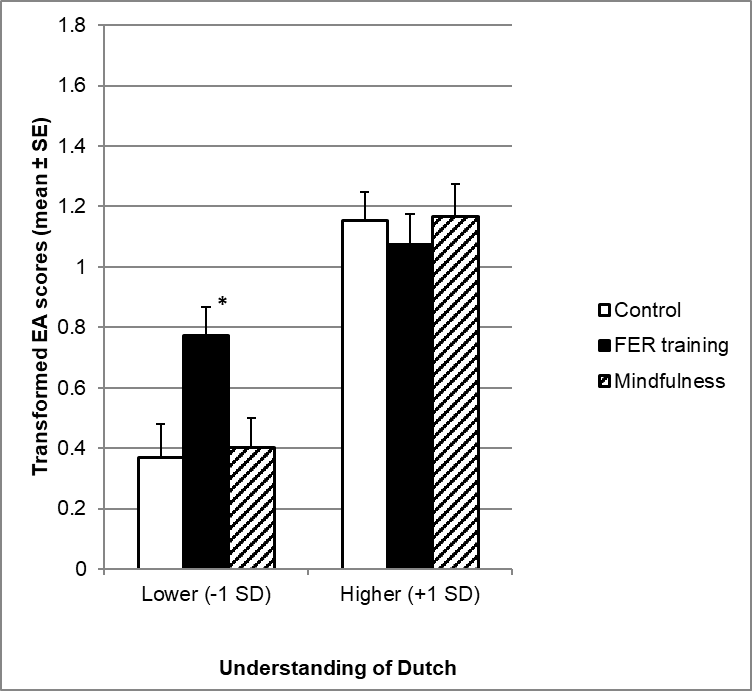
\includegraphics[width=\columnwidth]{media/image1.png} 
\caption{The Experimental Setup \hspace{\textwidth}
\emph{Participants were given a bag with 50 black socks and 40 brown socks \emph{(panel a)}. The researcher stayed in the room to give instructions and make notes \emph{(panel b)}.}} 
\label{fig:figure1}
\vskip-3pt
\end{figure}

Participants were filmed in a purposely-built lab with three in-built cameras to facilitate coding for the behavioral hypothesis. To minimize the differences between the conditions, both high- and low-interactivity conditions had the same initial setup: In both conditions, each participant was presented with a bag of 90 socks, among which were 50 black and 40 brown, and the only difference was that participants in the high-interactivity condition were allowed to pull socks from the bag (see Figure \ref{fig:figure1}). 




The original instructions ran thus: ``If you have a drawer with brown socks and black socks mixed in a ratio of 4:5, how many would you have to pull out in order to guarantee a pair?'' The instructions were read aloud to participants. However, after piloting, these needed to be refined and the final instructions ran thus: "In this bag are brown socks and black socks in a ratio of 4 brown socks for every 5 black socks\ldots{} so the ratio of brown socks to black socks is 4 to 5, \emph{is that clear}? What is the minimum number of socks you think you need to take out of the bag at random to be sure you had a pair of either brown sock or back socks, so that is if you were to pull socks out at random from the bag, what is the minimum number of socks that you would need to be sure that you would have one pair, \emph{that's two socks which match in color,} whether that's one pair of brown socks or one pair of black socks."

Participants were given 5 minutes to answer the problem and they were allowed to make multiple attempts. They were not prevented from speaking to the researcher nor, however, were they requested to follow a think-aloud protocol. The researcher would only answer questions by repeating the relevant part of the instructions. The researcher kept detailed notes while observing the participants; the participants were recorded throughout the study and the videos were later watched and coded. The participants' performance was measured in terms of success and the latency to a correct solution. 

\addcontentsline{toc}{subsection}{Results}
\subsection*{Results}

Performance was better in the high-interactivity condition in which 10 participants (or 50\%) solved the problem compared to the low condition in which 7 participants (or 38\%) did so. This difference was not significant, however ($\chi^2$(1, \emph{N} = 38) = 0.47, \emph{p} = .492, Cramer's V = 0.11). Participants were slower in the high-interactivity condition with an average latency of 116.20 seconds (\emph{SD} = 78.67; although this was skewed by participant 41 who took 297 seconds) than in the low condition (\emph{M} = 103.57 s, \emph{SD} = 48.32, which was skewed by participant 18 who announced the answer immediately, hence with a latency of 0; see Figure \ref{fig:figure2}); this difference was not significant, \emph{t}(15) = 0.38, \emph{p} = .713, Cohen's \emph{d} = 0.19. Removing these two outlying participants, the mean latencies were 96.1 s (\emph{SD} = 49.4) and 120.8 s (\emph{SD} = 17.3) in the high- and low-interactivity conditions respectively (\emph{t}(13) = 1.167, \emph{p} = .264, Cohen's \emph{d} = 0.82). 


\begin{figure}[t]
\vskip6pt
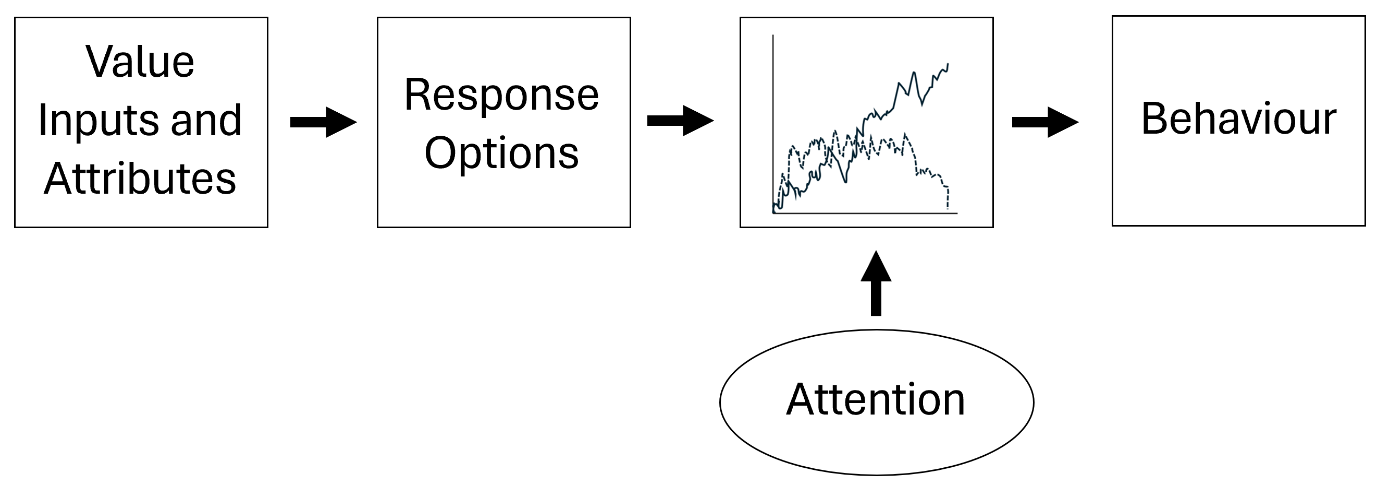
\includegraphics[width=\columnwidth]{media/image2.png}
\caption{\emph{Latency to Solution in Seconds} }
\label{fig:figure2}
\vskip-.4\baselineskip
\end{figure}


\addcontentsline{toc}{section}{Qualitative Section}

\section*{Qualitative section}
\vskip\baselineskip
\addcontentsline{toc}{subsection}{Method}
\subsection*{Method}

Over the course of the research, it became clear that the experimental manipulation failed and that there were significant procedural and theoretical assumptions and errors. Some were failures in experimental procedures\footnote{ In this respect, filming the experimental situation is a useful tool to ensure adherence to a set experimental procedure. In this instance, there was only one researcher but in other cases there may be multiple researchers. Given that we are still unclear of the contextual variables that may influence results (\nptextcite[]{Leonelli2018}), generating open-ended data is necessary to understand the complexity.} which could be rectified in a second study, but as we will see, others undermined the initial premise of the study and led to the decision to not repeat the study. 

Additionally, the video data suggested that there were underlying patterns from which new knowledge about this problem situation could be deduced beyond that contained within the structures of the hypothetico-deductive model. In other words, theoretically valid reasons for the practical and experimental failure of the experiment could be seen in the behavior of participants throughout the experimental situation. A decision was made to employ a modified version of Grounded Theory Method (GTM; \nptextcite[]{Glaser1967}) with the video data to generate novel theories about problem-solving in this task. Thus, the focus of the research shifted from an experimental manipulation to an observational study assessing qualitatively how participants solve this problem. Consequently, we abandoned the original hypotheses. 
\vskip3pt
\addcontentsline{toc}{subsubsection}{Analytical Process}
\subsubsection*{Analytical process}

The initial observations generated \textit{in vivo} were followed up by a close examination of the video data with time-stamped qualitative memos. Conversations were transcribed and time stamped. These observations were then grouped into conceptual categories before the videos were reviewed a second time to substantiate these categories. This iterative process continued through initial drafts of this paper. In tandem with the data analysis carried out through watching the videos, results were discussed between both authors and conceptual categories were refined. 

\addcontentsline{toc}{subsection}{Results}
\subsection*{Results}

The initial hypothesis of an augmentative effect of a high-interactivity environment compared to a low-interactivity environment was not sustained. The qualitative analysis detailed below pinpoints why this might be so: Excess environmental information and the encouragement to interact with it reified unhelpful representations. Additionally, a form of \emph{social} and \emph{linguistic} interactivity which focused on the instructions and the researcher replaced the object-based interactivity. The iterative process of discovery emerged more often in this linguistic space than in the space between object and person. This was a form of interactivity that was not accounted for in the rather narrow (and, in hindsight, naïve) high- and low-interactivity conditions outlined above, and yet it occurred in both experimental conditions and was in part the reason for the inconclusive results and the failed manipulation. 

\addcontentsline{toc}{subsubsection}{Information in the Environment}
\subsubsection*{Information in the environment}

The socks problem is a hard one because participants get stuck on the unhelpful ratio. As suggested by \textcite{Vallee-Tourangeau2020}, ignoring the ratio should lead to participants solving the problem more often and faster because they are not tempted to use inappropriate mathematical formulae. As we have addressed above, this is not an unreasonable assumption. However, the specific hypothesis under exploration, that a high-interactivity environment would increase the number of people who disregard the ratio, was not sustained by an analysis of what people did in this condition; it appeared that the opposite was the case, that a high-interactivity reinforced the unhelpful information. 

There are two ways in which a problem-solver could approach solving a problem using interactivity: The first involves the sort of exaptative actions mentioned in the initial hypothesis, while the second involves using the world to scaffold existing representations. In the case of problems designed to elicit an unhelpful representation, it is plausible that such a representation, when reified, would be harder to disregard. A high-interactivity environment can scaffold unhelpful representations as well as helpful ones. 

This reification was clearly in line with evidence in the study reported here: Interactivity allowed participants to represent the ratio in a solid form. Many of them pulled five brown socks from the bag and then four black socks and used these to structure their thoughts, so the ratio became harder to disregard. This was a sensible decision; it is not unreasonable to assume that the information in the problem is important (in terms of conversational pragmatics, it would make little sense to be informed of the ratio if it was not relevant; \nptextcite[]{Grice1975}). Therefore, the strategy of reifying the ratios is on the one hand sensible, and paradoxically, on the other hand, makes the problem harder to solve. 

However, in addition to allowing the reification of the information in the problem, the presentation of actual socks expanded the amount of information and the number of possible unproductive pathways. Problem-solving in this less controlled environment did not scaffold thought but rather created an additional distraction. Indeed, the concrete anchoring of the problem led people to look at the distribution of socks in the \emph{actual} bag that they had in front of them rather than considering it an abstracted entity. This was true even for those who were in the low-interactivity condition who tended to return their gaze to the bag when thinking. Take for example, participant 36: Figure \ref{fig:figure3} demonstrates the extent to which she was looking at and into the bag even while not interacting with the socks in it. Throughout the course of the experiment, she looked at the bag and the accompanying finger gestures and mouthing of numbers indicate that she was trying to count the socks that were in it. 

So, rather than supporting problem-solving, the actual physical arrangements of socks added complexity. Participant 26 (low-interactivity) said ``Well looking at \emph{this} bag, all the black socks are at the top so it would take a while to get a brown pair'' (01:36). Within a traditional problem-solving environment, participants know that they are solving a riddle and that they are in an artificial situation. In this experiment, the artificial, almost school-type problem collapsed with the far too mundane situation of finding a pair of socks. There simply is no ``real-world'' version of the hypothesized riddle. Somehow, the simplicity of this quotidian activity supported the intractability of the mathematical puzzle: If you want a pair of socks, you get them out of the bag. 


\begin{figure}

\vskip5pt
 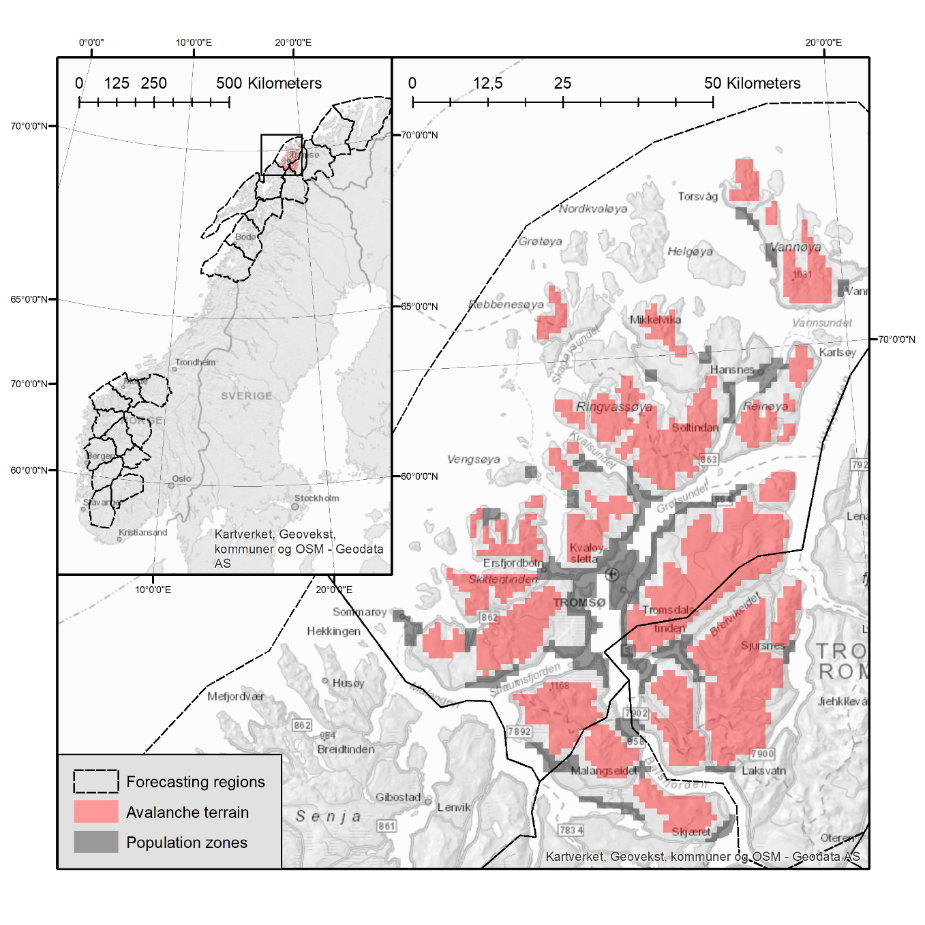
\includegraphics[width=\columnwidth]{media/image3.png} 
\caption{The first minute of participant 36 considering the problem. \emph{Stills were taken at the start of the task and every 10 seconds thereafter.}}
\label{fig:figure3}
\vskip7pt
\end{figure}


Additional information was deeply unhelpful in this case. When the problem is presented as a verbal riddle, the number of socks is not given; not only is there no way of knowing it, it is also irrelevant. However, when the participants are presented with a bag full of socks and a problem masquerading as a mathematical one, the total number of socks appears to take on more importance, much like the ratio information in the verbal form of the puzzle. In addition, investigating this unproductive cul-de-sac was easier for those in the high-interactivity condition and therefore harder to disregard. Take for example participant 37: After asking for clarification of the problems at 33 seconds into the task, he asked: ``How many were there in total?'' (00:33). After 58 seconds elapsed, he decided to empty the bag and to count the socks. It is hard to overstate what a poor decision this is (illustrated in Figure \ref{fig:figure4} where a screenshot was taken every 10 seconds over the following 220 seconds). Perhaps like participant 25, who stated ``Ah, that's what I have to do, I have to know how many are in here'' (02:15) before tipping the bag out, the participant thought he had solved the ``trick''. Whatever the reason, the messiness of tipping out all the socks then counting them and the high time cost meant that he made no progress. This wrong route would not have been possible in a low-interactivity or second-order problem-solving environment, yet again it is important to stress that this is not an illogical decision. 


\begin{figure*}
\centering
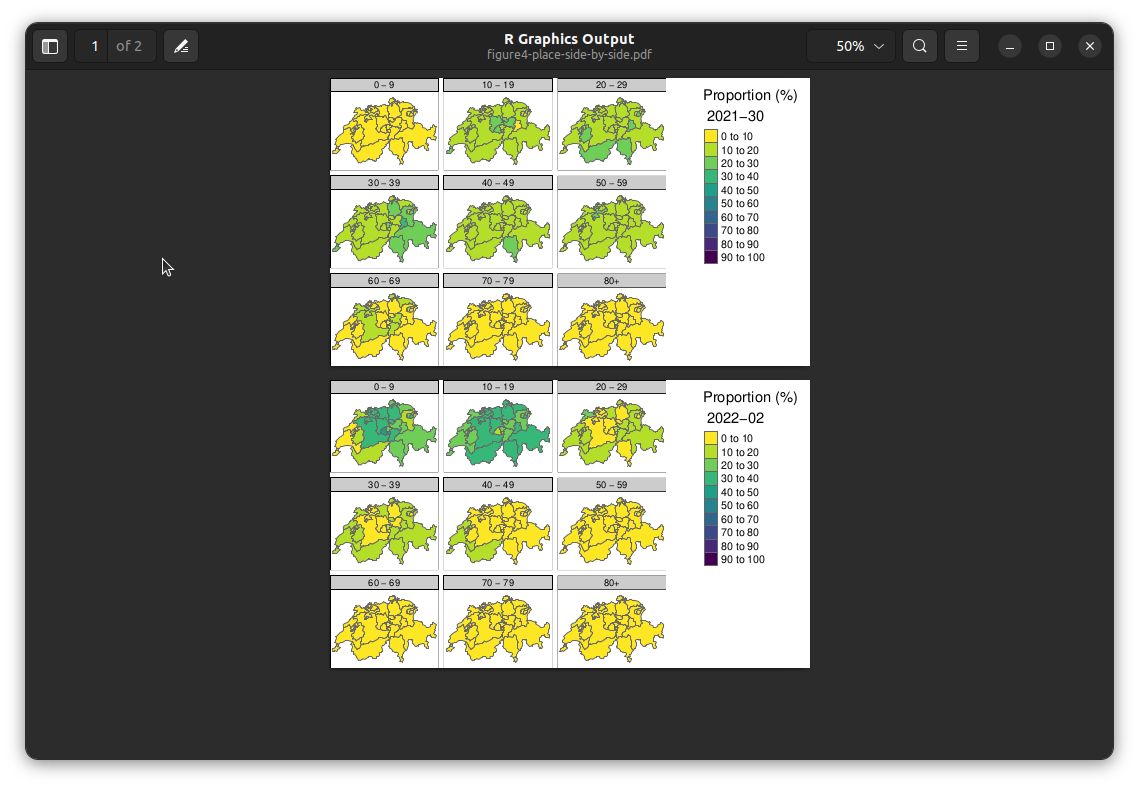
\includegraphics[width=5.25905in,height=8.51806in]{media/image4.png} 
\caption{Participant 37 tidying socks. \emph{Stills were taken at 60 seconds and every 10 seconds thereafter.}}
\label{fig:figure4}
\end{figure*}



\addcontentsline{toc}{subsubsection}{Porous Cognitive Boundaries}
\subsubsection*{Porous cognitive boundaries}

Additionally, the video data revealed versions of cognitive interactivity which were not related to the moving of the objects and hence did not feature in the original hypotheses but which scaffolded the pathway to solution. For instance, the instructions played a critical role in this scaffolding. This was an unintended artifact of the experimental situation and, albeit subsequently serendipitous, an inelegant one. The instructions were given verbally, and the participants were allowed to ask for clarification. The clarification took the form of the experimenter repeating the relevant set of instructions. Thus, what is often unspoken (checking instructions) became a traceable experimental artifact. 

What this underscored was the importance of the instructions to the problem solution. Initially, there was a change made to the instructions, as outlined above, to ensure that all salient information was clearly presented, but this did not change the participants' need for clarification. This clarification revealed two things: First, a consistent epistemic state across participants despite consistent task instructions should not be assumed; second, it was possible to use these clarifications in a trial-and-error way to structure understanding and gain new knowledge. Indeed, the nature of the task requires restructuring the instructions rather than manipulating the visuospatial field. Therefore, it is not unreasonable that the interactivity coalesces on this linguistic plane. 

The verbal nature of the instructions also increased interaction with the researcher. This was unanticipated in the original research design and invited the researcher into the experimental situation in a way normally avoided in experimental psychology. What these interactions revealed was the need for the participant to seek help from the outside world. Over the course of these interactions, the answer often revealed itself through a gradual recursive dialogical process. Taking for example participant 41 (Table \ref{tab:table1}), the last minute or so of her problem-solving involved a recursive, back-and-forth between extracting information from the socks that she had in her hand, the instructions, and the researcher through making guesses until she suggested the correct answer. Note how often she looked at the researcher and solicited feedback in the episodes selected. In this case, the playing with socks coupled with the information from the researcher and the redrawing of the epistemic map through the wrong guesses scaffolded the way to a solution. 

\begin{table*}[ht!] \sffamily
  \rowcolors*{3}{}{}%
\caption{Participant 41 solving the problem. \hspace{\textwidth}
\emph{The timestamps for Table \ref{tab:table1} and Table \ref{tab:table2} refer to the time from the start of the instructions. }}
\label{tab:table1}
\begin{mdframed}[linecolor=jotedark]
\vskip4pt
\renewcommand{\arraystretch}{2.5}
\begin{tabularx}{\linewidth}{@{} m{.05\linewidth} m{.2\linewidth} >{\raggedleft\arraybackslash}m{.19\linewidth}  m{.05\linewidth} m{.2\linewidth} >{\raggedleft\arraybackslash}m{.19\linewidth} }

\textbf{04:53}  &  Pulls out two more - this time both black  &  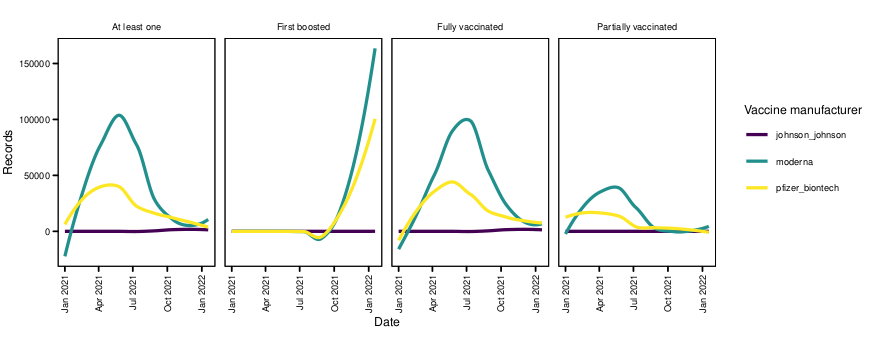
\includegraphics[height=.15\textheight, width=.8\linewidth]{media/image5.png}  &
 \textbf{05:35} & "So I could pull out four socks and then two would be a pair" & 
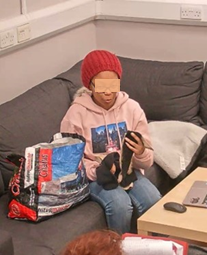
\includegraphics[height=.15\textheight, width=.8\linewidth]{media/image10.png}  \\
 \textbf{05:07} & "This is 8....." & 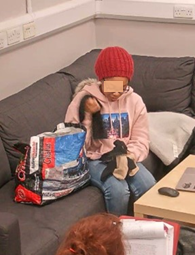
\includegraphics[height=.15\textheight, width=.8\linewidth]{media/image6.png} &
 \textbf{05:42} & Researcher repeats request for the \emph{minimum number} & 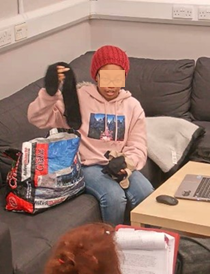
\includegraphics[height=.15\textheight, width=.8\linewidth]{media/image11.png} \\ 
 \textbf{05:08} & Looks at researcher & 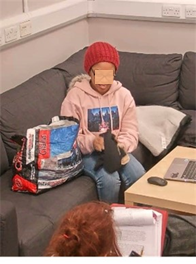
\includegraphics[height=.15\textheight, width=.8\linewidth]{media/image7.png} &
 \textbf{05:45} & Plays with socks in her hand & 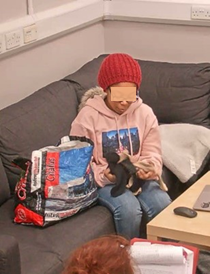
\includegraphics[height=.15\textheight, width=.8\linewidth]{media/image12.png} \\
 \textbf{05:14} & Pulls through socks in hands & 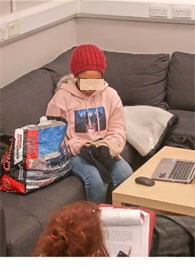
\includegraphics[height=.15\textheight, width=.8\linewidth]{media/image8.png} &
  \textbf{05:50} & "Three" & 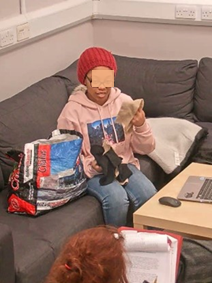
\includegraphics[height=.15\textheight, width=.8\linewidth]{media/image13.png} \\
 \textbf{05:21} & "So I have to pull out a pair?" & 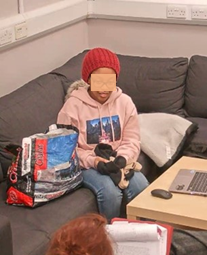
\includegraphics[height=.15\textheight, width=.8\linewidth]{media/image9.png} &
 \textbf{05:57} & Correct explanation & \\
 \textbf{05:23} & Researcher repeats instructions & \\ 

\end{tabularx} 
\vskip4pt
\end{mdframed}
\end{table*}

This was even clearer in the low-interactivity condition where the participants sought out scaffolding more obviously. Take for example, participant 26 in Table \ref{tab:table2}. This was a low-interactivity participant who uncovered the answer through a series of guesses using the feedback as a scaffold. As she stated clearly when asked if she knows why: "When I got to the end I did...when I said two and then I realized..." (02:51). The act of saying the word alongside the feedback from the environment scaffolded her understanding. Knowledge was gained when the thought was in the world; even if that realization did not take material form, it was still generated in action, this time the action of guessing. To place the results from this participant in a low-interactivity environment would be misleading even if she did not carry out any actions on any objects.

\begin{table*}[ht!] \sffamily
  \rowcolors*{3}{}{}%
\caption{Participant 26 solving the problem through incremental guessing}
\label{tab:table2}
\begin{mdframed}[linecolor=jotedark]
\renewcommand{\arraystretch}{1.5}
\begin{tabularx}{\linewidth}{@{} p{.05\linewidth} p{.28\linewidth} >{\raggedleft\arraybackslash}p{.1\linewidth}  p{.05\linewidth} p{.28\linewidth} >{\raggedleft\arraybackslash}p{.1\linewidth} @{}}
 \textbf{01:18}  & "Oh what and if I get it right you'll tell me?"  &  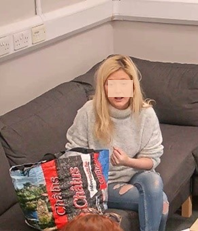
\includegraphics[height=.09\textheight, valign=t]{media/image14.png}  &
 \textbf{02:17} & "I'd have to pick 8 socks outs" & 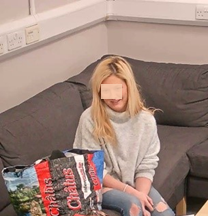
\includegraphics[height=.09\textheight, valign=t]{media/image22.png} \\ 
 
\textbf{01:21} & "Hang on, I don't know how many socks are in the bag?" & 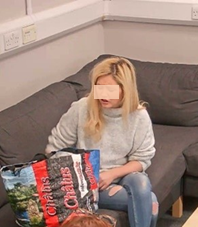
\includegraphics[height=.09\textheight, valign=t]{media/image15.png} & 
 \textbf{02:23} & "I'd have to pick 20 socks out" & 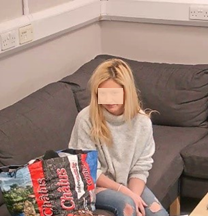
\includegraphics[height=.09\textheight, valign=t]{media/image23.png} \\ 
 
\textbf{01:24} & Looks at researcher expectantly. & 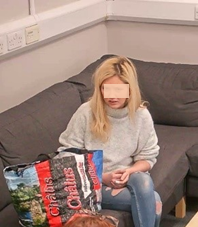
\includegraphics[height=.09\textheight, valign=t]{media/image16.png} &
 \textbf{02:32} & "I'd have to pick 18 socks out" & 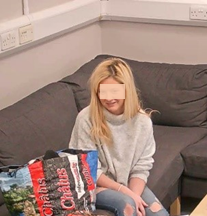
\includegraphics[height=.09\textheight, valign=t]{media/image24.png} \\ 
 
\textbf{01:27} & "So I don't get how the ratio would matter if I don't know how many socks were in the bag....oh. it's just chance isn't it?" & 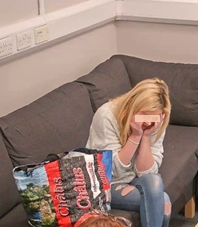
\includegraphics[height=.09\textheight, valign=t]{media/image17.png} &
 \textbf{02:41} & "I'd have to pick 4 socks out". Said faster and more determined & 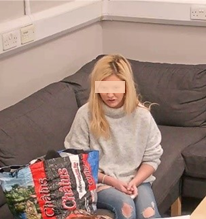
\includegraphics[height=.09\textheight, valign=t]{media/image25.png} \\ 
 
\textbf{01:36} & "Well, looking at the bag actually all the black ones are on top so it might be a while to get a pair of brown ones.." & 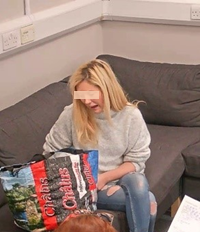
\includegraphics[height=.09\textheight, valign=t]{media/image18.png} &
 \textbf{02:44} & "2 socks" & 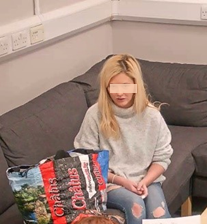
\includegraphics[height=.09\textheight, valign=t]{media/image26.png} \\ 
 
\textbf{01:45} & "I'm so confused by the question" Looks at researcher again & 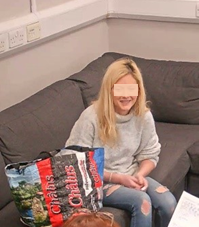
\includegraphics[height=.09\textheight, valign=t]{media/image19.png} &
  \textbf{02:47} & "3 socks" & 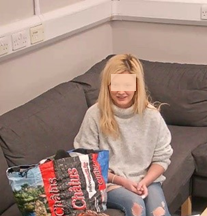
\includegraphics[height=.09\textheight, valign=t]{media/image27.png} \\ 

\textbf{01:47} & Researcher repeats instructions &  &
 \textbf{02:49} & Researcher confirms & \\
 
\textbf{01:50} & Starts to pull socks; Researcher stops her & 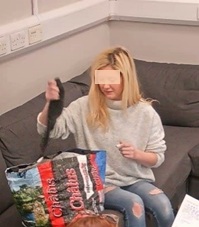
\includegraphics[height=.09\textheight, valign=t]{media/image20.png} &
 \textbf{02:50} & Starts to laugh & \\ 
 
 \textbf{02:03} & Researcher ends instructions & &
 \textbf{02:51} & "When I got to the end I did...when I said 2 and then I realized...." & 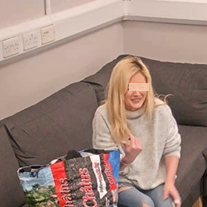
\includegraphics[height=.09\textheight, valign=t]{media/image28.png} \\ 
 
 \textbf{02:11} & "I'd have to pick 10 socks out" & 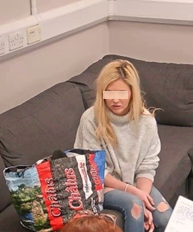
\includegraphics[height=.09\textheight, valign=t]{media/image21.png} & & &\\
\end{tabularx}
\vskip4pt
\end{mdframed}
\end{table*}




\addcontentsline{toc}{subsection}{Discussion}
\subsection*{Discussion}

The quantitative results were inconclusive. It may be that if the study had reached the anticipated number of 60 participants, they would show a significant augmentative effect of interactivity, but that seems unlikely. Moreover, the cognitive messiness of the procedure would mean that it would be hard to trust that the results reflected the experimental manipulation, that is, one group of participants interacting with the physical model of the problem, and one group interacting with no features of the task environment, including with the researcher! Of course, the problems outlined above would cast the experiment as a failure by the standards of traditional experimental psychology. As argued by \textcite{Gozli2017}, the experiment in psychology takes the form of rule-governed behavior. In the experiment reported here, the participants did not play by the rules of the experiment, namely to use only mental simulations in the low-interactivity, sequestered condition and to usefully employ the objects in the high-interactivity condition. Thus, the experimental manipulation and the experiment failed. 

It would be possible, of course, to design a low-interactivity task environment where interaction with the experimenter was completely removed beyond the initial task instructions (e.g., the experimenter could walk away from the observation lab and take their notes from the control booth). Accordingly, the high interactivity condition could be designed to force participants to take one sock at a time, instruct them to reflect on what they see, and prompt them to provide an answer to the puzzle after each draw. Such task procedures might improve the operationalization of the levels of interactivity envisaged in \textcite{Vallee-Tourangeau2020}'s original thought experiment. Be that as it may, the data reported here unveil the affordances offered by the elements of the wider system, and the felicitous (such as soliciting feedback dialogically in the low-interactivity condition) and infelicitous outcomes (such as reifying the 4:5 ratio in the high-interactivity condition) that result from the participants' actions. Such an analysis is likely to yield a greater understanding of how problem-solving unfolds in more complex situations. 

The qualitative analysis undertaken here also offers an understanding of the detrimental role that interactivity can play alongside the traditionally-theorized augmentative role. In hindsight, such an effect is theoretically more plausible given an open cognitive system and a non-computational approach. The data presented here suggest that a cognitive system forms around any problem-solver and that once we approach cognition from this systemic perspective, we necessarily introduce multiple shifting parts. Here, when interactivity with the objects proved to be unhelpful, cognition seeped out into the wider system to encompass the interaction with the researcher via the instructions. These observations license two broader comments on the nature of experimental research in interactivity: (a) on problem-solver omniscience and (b) on the inherently contingent nature of wide cognition. 

\addcontentsline{toc}{subsubsection}{The Omniscient Problem-Solver}
\subsubsection*{The omniscient problem-solver}
\vskip3pt
Problem-solving is broadly the movement from a state of ignorance to a state of knowledge (\nptextcite[]{Arfini2021}). There are two forms this ignorance can take, ignorance of the process of problem solution or ignorance of the answer. The most efficient pathway to a solution can only be directly and easily enacted when the solution is already known and can be traced backward without the risk of a false start or a complete divergence from the path. This requires foreknowledge of the correct answer, which is a paradoxical situation and assumes an omniscient problem-solver. 

For analytical problems, while the answer is unknown, the process of getting to the answer is clear and known. For example, for mental arithmetic, while the problem-solver may not know the solution, they will know the most efficient process and the simple operators to evince it.\footnote{Indeed, the accuracy of the solution is not clear in itself but is predicated on an accurate following of the steps. We only trust an answer to a mental arithmetic problem not because of the answer itself but because we trust in the steps that led to the answer.} These steps will have been predetermined culturally and through personal experience. Therefore, it is likely that the agent will select the correct objects and the correct actions over those objects. This means that an agent-centric model of interactivity should yield supportive empirical data. However, it is unclear how far such a model would extend. In many ill-structured problems or non-analytical problems, the problem-solver is in double ignorance: They do not know the correct solution or the manner of approaching the correct solution. In terms of problem-solving with and through objects, this means that they will not necessarily select the correct objects or actions over them but merely those that satisfy the needs at the time (echoing the Criterion of Satisfactory Progress Theory; \nptextcite[]{MacGregor2001,Ormerod2013}). Without omniscience, the problem-solver can make logical and plausible moves that lead them further from the problem solution. 
\vskip2pt
\addcontentsline{toc}{subsubsection}{Wide Cognition Is Contingent}
\subsubsection*{Wide cognition is contingent}

The components in complex systems interact in complex ways and the results are emergent and contingent. Pre-specification of underlying causal mechanisms is difficult because adhering to a form of wide cognition (see \nptextcite{Wilson2009}) means that such pre-specification is necessarily an under-specification: It is impossible to predict in advance which solution routes will be useful, especially if that problem solution is generated by unplanned and exaptative gestures, which is more likely in materially rich environments. It suggests that in insight tasks where there is a double ignorance---ignorance of the solution and ignorance of the path to the solution---both the finding of the solution and the path taken become important. 

Interactivity posits that a dynamic relationship with the external world is not only augmentative to cognition processes but necessary. However, experimental research in interactivity does so by paradoxically setting up a low-interactivity condition which admits non-interactive thinking. In this way, it assumes that there is an easy way to compare non-systemic and systemic cognition and that non-systemic cognition can be meaningfully isolated in an experimental psychologist's lab. We suggest that the dualistic assumptions underlying this approach are misguided, as they assume an ideal type of experimental participant can be generated in sequestered experimental conditions. Rather, the evidence we present here suggests a cognitive leakage across both experimental conditions. In the process of operationalizing the so-called low-interactivity condition, the presence of the experimenter offered an external resource with which to scaffold the problem-solving process. The participant naturally transformed a solo and ostensibly unaided effort into a dyadic one. Clearly, the experimenter qua interlocutor was an unrequited conversational partner. Still, in the absence of hard physical or instructional constraints, the participant naturally availed themselves of this resource, bootstrapping the cognitive effort through a dialogue with their reluctant partner. And it is through this dialogue that the participant's hunch underwent many different forms until it was eventually translated into the normative one. These ersatz dialogues offer a telling window into the distributed nature of thinking, in this instance, the distribution over time and the gradual sedimentation through iterative dialogical cycles. The reification of the solution was the product of interactivity despite the experimental procedure. 

A systematic approach to cognition requires that every thoughtful (and arguably every non-thoughtful) encounter should be analyzed as part of a system; however, what constitutes part of the system is rarely specified. \textcite{Vallee-Tourangeau2020} suggest that a cognitive ecosystem is configured by ``the reasoner, the physical reality of the problem, and the action possibilities offered by the external environment'' (p. 826). We argue that the data here suggest ``the action possibilities offered by the external environment'' (p. 826) are broader than whether the problem is represented in movable artifacts or not. Rather, participants actively recruit beyond the resources of interest in the experimental conditions. This means a more granular approach needs to be considered. 

\addcontentsline{toc}{subsubsection}{Conclusion}
\subsubsection*{Conclusion}

The data presented here are not the clean data typically seen in psychological reports of experimental situations. Over the course of the study, a more ethnographic approach to the whole experimental situation provided rich data about different types of interactions that emerged in either a so-called low- or high-interactivity condition. Some aspects are unique to the situation of an exploratory, quasi-pilot study in problem-solving and others are broader reflections on the nature of research in psychology. As we have seen above, the transformation from a sequestered condition to a more ``real-life'' situation does not necessarily occur without cost and the nature of that cost deserves to be explored. Additionally, it casts doubt on the possibility of creating a fully sequestered condition. Rather, the data presented here suggest that both conditions are porous. 

The failure of the experimental procedure here revealed the difficulty of doing research in open cognitive systems. Traditional methods of assessing embedded or extended cognition are still rooted in a cognitive and computational model of mind and contrast low- and high-interactivity environments to demonstrate an augmentative effect of interactivity. The research presented here suggests that the reality of experimenting in an open system is more complex than is believed. The target problem here was designed as a mental riddle and its transposition to an interactive space offered a telling window into the disconnect between first- and second-order problem-solving: The task only ``works'' as a second-order task. 

It is tempting to question whether the mental tasks used in traditional cognitive psychology experiments~are diagnostic of problem-solving~outside of the sequestered~laboratory environments in which they are commonly operationalized. We propose, rather, that a research program should develop in parallel to examine the solving of problems which are rendered complex not because of their structure but because of their situation. When it comes to problem-solving, we need a wider range of outcome measures to even begin to understand how it unfolds across a range of contexts, which requires a combination of qualitative and quantitative work. What we can see here is that the genesis of a new idea involves a transformation, which in turn involves resources; these resources come with a cost, and these transactions leave physical traces which can be mapped. To understand the transformations and transactions, that is, the process through which new ideas are constructed, the analysis must be local and granular. It is our belief that turning to the qualitative in cognitive psychology to complement the quantitative will yield great benefits. 

\printbibliography
\newpage


\section*{License}
        \begin{wrapfigure}[2]{L}{0.08\textwidth}%
        \vspace{-12pt}
        
\includegraphics[width=0.1\textwidth]{media/by}%
        \end{wrapfigure}
        \textbf{Open Access} This article is licensed under a Creative Commons Attribution 4.0 International License, which permits use, sharing, adaptation, distribution and reproduction in any medium or format, as long as you give appropriate credit to the original author(s) and the source, provide a link to the Creative Commons license, and indicate if changes were made. The images or other third party material in this article are included in the article’s Creative Commons license, unless indicated otherwise in a credit line to the material. If material is not included in the article’s Creative Commons license and your intended use is not permitted by statutory regulation or exceeds the permitted use, you will need to obtain permission directly from the copyright holder. To view a copy of this license, visit \href{https://creativecommons.org/licenses/by/4.0/}{https://creativecommons.org/licenses/by/4.0/}.
        \newline\newline
        \textcopyright \text{ }Ross \&  Vallée-Tourangeau 2021
\end{document}